\documentclass{article}
\usepackage[margin=1in]{geometry}
\usepackage{hyperref}
\usepackage{amsmath,amsfonts,amssymb,amsthm,commath,dsfont}
\usepackage{enumitem}
\usepackage{framed}
\usepackage{xspace}
\usepackage{microtype}
\usepackage{float}
\usepackage[round]{natbib}
\usepackage{cleveref}
\usepackage[dvipsnames]{xcolor}
\usepackage{graphicx}
\usepackage{listings}
\usepackage[breakable]{tcolorbox}
\tcbset{breakable}
\usepackage{mathtools}

\newcommand{\colbar}{\rule[-3mm]{.3mm}{1.5em}}
\newcommand{\rowbar}{\rule[.5ex]{1.5em}{.3mm}}
\DeclareMathOperator{\rank}{rank}

% following loops stolen from djhsu
\def\ddefloop#1{\ifx\ddefloop#1\else\ddef{#1}\expandafter\ddefloop\fi}
% \bbA, \bbB, ...
\def\ddef#1{\expandafter\def\csname bb#1\endcsname{\ensuremath{\mathbb{#1}}}}
\ddefloop ABCDEFGHIJKLMNOPQRSTUVWXYZ\ddefloop

% \cA, \cB, ...
\def\ddef#1{\expandafter\def\csname c#1\endcsname{\ensuremath{\mathcal{#1}}}}
\ddefloop ABCDEFGHIJKLMNOPQRSTUVWXYZ\ddefloop

% \vA, \vB, ..., \va, \vb, ...
\def\ddef#1{\expandafter\def\csname v#1\endcsname{\ensuremath{\boldsymbol{#1}}}}
\ddefloop ABCDEFGHIJKLMNOPQRSTUVWXYZabcdefghijklmnopqrstuvwxyz\ddefloop

% \valpha, \vbeta, ...,  \vGamma, \vDelta, ...,
\def\ddef#1{\expandafter\def\csname v#1\endcsname{\ensuremath{\boldsymbol{\csname #1\endcsname}}}}
\ddefloop {alpha}{beta}{gamma}{delta}{epsilon}{varepsilon}{zeta}{eta}{theta}{vartheta}{iota}{kappa}{lambda}{mu}{nu}{xi}{pi}{varpi}{rho}{varrho}{sigma}{varsigma}{tau}{upsilon}{phi}{varphi}{chi}{psi}{omega}{Gamma}{Delta}{Theta}{Lambda}{Xi}{Pi}{Sigma}{varSigma}{Upsilon}{Phi}{Psi}{Omega}{ell}\ddefloop

\newcommand\T{{\scriptscriptstyle\mathsf{T}}}
\def\diag{\textup{diag}}

\DeclareMathOperator*{\argmin}{arg\,min}
\DeclareMathOperator*{\argmax}{arg\,max}

\def\SPAN{\textup{span}}
\def\tu{\textup{u}}
\def\R{\mathbb{R}}
\def\E{\mathbb{E}}
\def\Z{\mathbb{Z}}
\def\be{\mathbf{e}}
\def\nf{\nabla f}
\def\veps{\varepsilon}
\def\cl{\textup{cl}}
\def\inte{\textup{int}}
\def\dom{\textup{dom}}
\def\Rad{\textup{Rad}}
\def\lsq{\ell_{\textup{sq}}}
\def\hcR{\widehat{\cR}}
\def\hcRl{\hcR_\ell}
\def\hcRlog{\hcR_{\log}}
\def\cRl{\cR_\ell}
\def\hcE{\widehat{\cE}}
\def\cEl{\cE_\ell}
\def\hcEl{\hcE_\ell}
\def\eps{\epsilon}
\def\1{\mathds{1}}
\newcommand{\red}[1]{{\color{red} #1}}
\newcommand{\blue}[1]{{\color{blue} #1}}
\def\srelu{\sigma_{\textup{r}}}
\def\vsrelu{\vec{\sigma_{\textup{r}}}}
\def\vol{\textup{vol}}
\def\vwols{\hat{\vw}_{\textrm{ols}}}
\def\llog{\ell_{\log}}
\newcommand{\pww}[1]{\hat p_{#1}}

\newcommand{\ip}[2]{\left\langle #1, #2 \right \rangle}
\newcommand{\mjt}[1]{{\color{blue}\emph\textbf{[M:}~#1~\textbf{]}}}
\newcommand{\sahand}[1]{{\color{green}\emph\textbf{[Sah:}~#1~\textbf{]}}}

\newtheorem{fact}{Fact}
\newtheorem{lemma}{Lemma}
\newtheorem{claim}{Claim}
\newtheorem{proposition}{Proposition}
\newtheorem{theorem}{Theorem}
\newtheorem{corollary}{Corollary}
\newtheorem{condition}{Condition}
\theoremstyle{definition}
\newtheorem{definition}{Definition}
\theoremstyle{remark}
\newtheorem{remark}{Remark}
\newtheorem{example}{Example}

\newenvironment{Q}
{%
  \clearpage
  \item
  }
  {%
    \phantom{s} %lol doesn't work
    \bigskip
    \textbf{Solution.}
  }

  \title{CS 446 / ECE 449 --- Homework 4}
  \author{\emph{acard6}}
  \date{Version 1.0}

  \begin{document}
  \maketitle

  \noindent\textbf{Instructions.}
  \begin{itemize}
    \item
      Homework is due \textbf{Tuesday, April 4, at noon CST}; no late homework accepted.

    \item
      Everyone must submit individually at gradescope under \texttt{hw4} and \texttt{hw4code}.

    \item
      The ``written'' submission at \texttt{hw4} \textbf{must be typed}, and submitted in
      any format gradescope accepts (to be safe, submit a PDF).  You may use \LaTeX, Markdown,
      Google Docs, MS Word, whatever you like; but it must be typed!

    \item
      When submitting at \texttt{hw4}, gradescope will ask you to mark out boxes/pages
      around each of your answers; please do this precisely!

    \item
      Please make sure your NetID is clear and large on the first page of the homework.

    \item
      Your solution \textbf{must} be written in your own words.
      Please see the course webpage for full academic integrity information.
      Briefly, you may have high-level discussions with at most 3 classmates,
      whose NetIDs you should place on the first page of your solutions,
      and you should cite any external reference you use; despite all this,
      your solution must be written in your own words.

    \item
      We reserve the right to reduce the auto-graded score for
      \texttt{hw4code} if we detect funny business (e.g., your solution
      lacks any algorithm and hard-codes answers you obtained from
      someone else, or simply via trial-and-error with the autograder).

    \item
      Coding problems come with suggested ``library routines''; we include these to reduce
      your time fishing around APIs, but you are free to use other APIs.

    \item
      When submitting to \texttt{hw4code}, only upload the two python files \texttt{hw4.py} and \texttt{hw4\_utils.py}. Don't upload a zip file or additional files.
      % Additional files will be ignored.

  \end{itemize}
  \noindent\textbf{Version history.}
  \begin{enumerate}
    \item Initial version.
  \end{enumerate}

  \begin{enumerate}[font={\Large\bfseries},left=0pt]
    \begin{Q}
  \textbf{\Large Linear Regression/SVD.}

  Throughout this problem let $\vX$ be the $n \times d$ matrix with the feature vectors $(\vx_i)_{i = 1}^n$ as its rows. Suppose we have the singular value decomposition $\vX = \sum_{i = 1}^r s_i \vu_i \vv_i^\top$.
  \begin{enumerate}
    \item Let the training examples $\del{\vx_i}_{i = 1}^n$ be the standard basis vectors $\ve_i$ of $\R^d$ with each $\ve_i$ repeated $n_i > 0$ times having labels $\del{y_{i_j}}_{j = 1}^{n_i}$. That is, our training set is:
    \[
        \bigcup_{i = 1}^d \cbr{\del{\ve_i, y_{i_j}}}_{j = 1}^{n_i},
    \]
    where $\sum_{i = 1}^d n_i = n$. Show that for a vector $\vw$ that minimizes the empirical risk, the components $w_i$ of $\vw$ are the averages of the labels $\del{y_{i_j}}_{j = 1}^{n_i}$: $w_i = \frac{1}{n_i}\sum_{j = 1}^{n_i} y_{i_j}$.
    
    \textbf{Hint:} Write out the expression for the empirical risk with the squared loss and set the gradient equal to zero.
    
    \textbf{Remark:} This gives some intuition as to why ``regression'' originally meant ``regression towards the mean.''
    
    \item Returning to a general matrix $\vX$, show that if the label vector $\vy$ is a linear combination of the $\cbr{\vu_i}_{i = 1}^r$ then there exists a $\vw$ for which the empirical risk is zero (meaning $\vX \vw = \vy$).
    
    \textbf{Hint:} Either consider the range of $\vX$ and use the SVD, or compute the empirical risk explicitly with $\vy = \sum_{i = 1}^r a_i \vu_i$ for some constants $a_i$ and $\hat{\vw}_{\textrm{ols}} = \vX^+ \vy$.
    
    \textbf{Remark:} It's also not hard to show that if $\vy$ is not a linear combination of the $\cbr{\vu_i}_{i = 1}^r$, then the empirical risk must be nonzero.
    
    \item Show that $\vX^\top \vX$ is invertible if and only if $(\vx_i)_{i = 1}^n$ spans $\mathbb{R}^d$.
    
    \textbf{Hint:} Recall that the squares of the singular values of $\vX$ are eigenvalues of $\vX^\top \vX$.

    \textbf{Remark:} This characterizes when linear regression has a unique solution due to the normal equation (note that we always have at least one solution obtained by the pseudoinverse). We would not have had a unique solution for part (a) if we had an $n_i = 0$.
    
    \item Provide a matrix $\vX$ such that $\vX^\top \vX$ is invertible and $\vX\vX^\top$ is not. Include a formal verification of this for full points.
    
    \textbf{Hint:} Use part (c). It may be helpful to think about conditions under which a matrix is not invertible.

    \textbf{Hint:}
    The ``formal verification'' doesn't need to be a lengthy proof: in particular, there exist choices of $\vX$ which are easy to write down,
    for which a verification of this claim is immediate.  It can also be beneficial to \emph{write down} the matrix directly via its SVD.
    
  %%%%%%%%%%%%%%%%%%%%%%%%%%%%%%%%%%%%%%%%$$my solutions for Q1. linear regression/SVD%%%%%%%%%%%%%%%%%%%%%%%%%%%%%%%%%%%%%%%%%%
  \end{enumerate}
  \end{Q}
  \begin{enumerate}
    \item each basis vector $e_{i}$ is repeated some $n_{i}$ times each repetition has their own label $y_{i,j}$ where $j \in \{0,n_{i}\}$.
    If $R(w) = \frac{1}{2n} \sum_{i=1}^{n} (w^{T}_{i}x_{i}-y_{i})^{2} 
    = \frac{1}{2n} \sum_{i=1}^{d} \sum^{n_{i}}_{j=1} (w^{T}_{i}x_{i}-y_{i_{j}})^{2}\\$ we substite in the basis vector $e_i$ for $x_i$ to get
    $w^Tx_i = w^T e_i = w_i$. Then we take the derivative w.r.t $w_i$ to get\\
    $\nabla_{w_{i}} R(w) = \frac{1}{n} \sum_{j=1}^{n_{i}} (w_i-y_{i_j})=0$. Since w is not dependent on j we can simplifiy\\ 
    $\frac{1}{n}(w_i - \sum_{j=1}^{n_i} y_{i_j}) = 0 \rightarrow \frac{1}{n} w_i = \frac{1}{n} \sum_{j=1}^{n_i} y_{i_j}$\\
    The mean of $w_i$ is 1 since there is only one value and the mean of $y_{i_j}$ is $\frac{1}{n_i}$ since it only depends on $n_i$, 
    thus finally giving us $w_i = \frac{1}{n_i} \sum_{j=1}^{n_i} y_{i_j}$

    \item $y=\sum_{i=1}^{r}a_i u_i$ for some const $a_i$. we want to show $\sum_{i=1}^r s_i u_i v_i^T w = \sum_{i=1}^{r}a_i u_i$. 
    This can be simplified to $\sum_{i=1}^r a_i v_i^T w s_i = \sum_{i=1}^{r}a_i u_i$. Adding in $s_i$ to give us the ith column of
    Xw and substiting $a_i$ with $s_i$.\\
    If $w = \sum_{i=1}^r \frac{a_i}{s_i} v_i \rightarrow$
    $\sum_{i=1}^r a_i v_i^T w s_i = \sum_{i=1}^r a_i v_i^T \left(\sum_{j=1}^r \frac{a_j}{s_j} v_j\right) s_i = 
    \sum_{i=1}^r \frac{a_i}{s_i} a_i s_i = \sum_{i=1}^r a_i^2$ and\\
    $\sum_{i=1}^r u_i a_i = \sum_{i=1}^r u_i \sum_{j=1}^r a_j \frac{s_j}{s_j} v_j^T u_i = \sum_{j=1}^r a_j v_j^T 
    \left(\sum_{i=1}^r u_i u_i^T\right) v_j = \sum_{j=1}^r a_j v_j^T v_j = \sum_{j=1}^r a_j$
    Therefore, $Xw = y$ and the empirical risk is zero.
    
    \item The key observation is that for $v \in \mathbb{R}^d, Xw=0$ if and only if $X^{T}Xw=0$.
    For the non-trivial implication, if $X^TXw=0$, then $w^TX^TXw=0$, that is $(Xw)^TXw=0$, which implies that $Xv=0$.
    If the rank of X is d, this means that X is one-to-one when acting on $\mathbb{R}^d$. 
    So by the observation, $X^TX$ is one-to-one, which makes it invertible (as it is square).
    Conversely, if the rank of X is less than m, there exists $w \in \mathbb{R}^d$ with $Xw=0$. Then $X^TXw=0$, and $X^TX$ cannot be invertible.
    
    \item Let us consider a 2x3 matrix where $X = \left[\begin{array}{ccc} 1 & 0 & 1 \\ 1 & 1 & 0 \end{array} \right]$ Then we have 
    $X^TX =  \left[\begin{array}{ccc} 2 & 1 & 1 \\ 1 & 1 & 0\\ 1 & 0 & 1 \end{array} \right]$ and 
    $XX^T = \left[\begin{array}{cc} 2 & 1\\ 1 & 2 \end{array} \right]$. The determinan for each is $det(XX^T) = 2$ and
    $det(X^TX) = 0$, since $X^TX$ is 0 it cannot have a determinant and is therefore not invertible, meanwhile $XX^T$ has 
    a nonzero determinant and thus is invertible. It can also be described by the fact that 
    $RREF(X^TX) = \left[\begin{array}{ccc} 0 & 0 & 0 \\ 1 & 1 & 0 \\ 1 & 0 & 1 \end{array} \right]$, having a rank of $2<d$ where d=3.
    $RREF(XX^T) = \left[\begin{array}{cc} 1 & 0 \\ 0 & 1 \end{array} \right]$ having a rank of 2=d where d=2
  \end{enumerate}



    \begin{Q}
      \textbf{\Large Linear Regression.}

      Recall that the empirical risk in the linear regression method is defined as $\hcR(\vw) := \frac{1}{2n}\sum_{i=1}^n (\vw^\top \vx_i - y_i)^2$, where $\vx_i \in \R^d$ is a data point and $y_i$ is an associated label.
      \begin{enumerate}
        \item Implement linear regression using gradient descent in the \texttt{linear\_gd(X, Y, lrate, num\_iter)} function of \texttt{hw4.py}. You are given as input a training set \texttt{X} as an $n \times d$ tensor, training labels \texttt{Y} as an $n \times 1$ tensor, a learning rate \texttt{lrate}, and the number of iterations of gradient descent to run \texttt{num\_iter}.  Using gradient descent, find parameters $\vw$ that minimize the empirical risk $\hcR(\vw)$. Use $\vw = 0$ as your initial parameters, and return your final $w$ as output. Prepend a column of ones to \texttt{X} in order to accommodate a bias term in $\vw$.

          \textbf{Library routines:} \texttt{torch.matmul (@), torch.tensor.shape, torch.tensor.t, torch.cat,} 

          \texttt{torch.ones, torch.zeros, torch.reshape}.

        \item Implement linear regression by using the pseudoinverse to solve for $w$ in the \texttt{linear\_normal(X,Y)} function of \texttt{hw4.py}. 
        You are given a training set \texttt{X} as an $n \times d$ tensor and training labels \texttt{Y} as an $n \times 1$ tensor. Return your parameters 
        $w$ as output. As before, make sure to accommodate a bias term by prepending ones to the training examples \texttt{X}.

          \textbf{Library routines:} \texttt{torch.matmul (@), torch.cat, torch.ones, torch.pinverse}.

        \item Implement the \texttt{plot\_linear()} function in \texttt{hw4.py}.  Use the provided function \texttt{hw4\_utils.load\_reg\_data()}\\ 
        to generate a training set \texttt{X} and training labels \texttt{Y}. Plot the curve generated by \texttt{linear\_normal()}\\ along with the 
        points from the data set.  Return the plot as output.  Include the plot in your written submission.

          \textbf{Library routines:} \texttt{torch.matmul (@), torch.cat, torch.ones, plt.plot, plt.scatter,}

          \texttt{plt.show, plt.gcf} where \texttt{plt} refers to the \texttt{matplotlib.pyplot} library.
      \end{enumerate}
    \end{Q}
    \begin{enumerate}
    \item[(c)] \begin{center}
      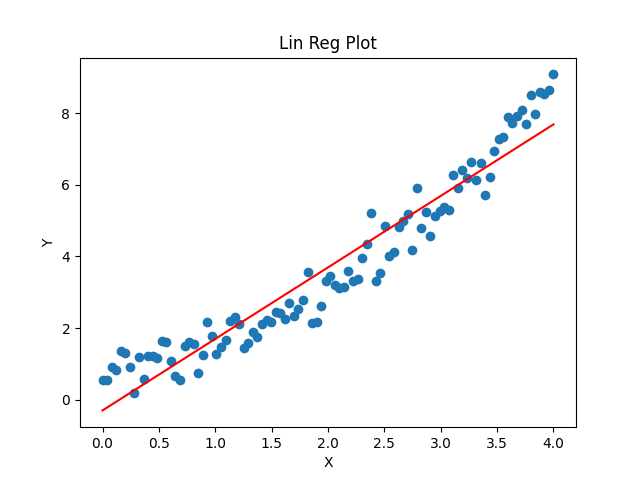
\includegraphics[scale=0.55]{lin_reg.png}\\
      \textbf{figure 1:} image of linear regression\\  
    \end{center}
  \end{enumerate}
    

    \begin{Q}
  \textbf{\Large Polynomial Regression.}

  In Problem 3 you constructed a linear model $\vw^\top \vx = \sum_{i=1}^d x_i w_i$.  In this problem you will use the same setup as in the previous problem, but enhance your linear model by doing a quadratic expansion of the features.  Namely, you will construct a new linear model $f_{\vw}$ with parameters
  \[
    (w_{0}, w_{01},\dots,w_{0d},w_{11}, w_{12},\dots,w_{1d},w_{22}, w_{23},\dots,w_{2d},\dots, w_{dd})^\top,
  \]
    defined by
  	\begin{align*}
  	f_{\vw}(x) = \vw^\top \phi(\vx) = w_0 + \sum_{i=1}^d w_{0i} x_i + \sum_{i\leq j}^dw_{ij} x_ix_j.
  	\end{align*}
  	
  \textbf{Warning:} If the computational complexity of your implementation is high, it may crash the autograder (try to optimize your algorithm if it does)!
  \begin{enumerate}
  \item Given a $3$-dimensional feature vector $\vx = (x_1,x_2,x_3)$, completely write out the quadratic expanded feature vector $\phi(\vx)$.
  \item Implement the \texttt{poly\_gd()} function in \texttt{hw4.py}.  The input is in the same format as it was in Problem 3.  Implement gradient descent on this training set with $\vw$ initialized to 0.  Return $\vw$ as the output with terms in this exact order: bias, linear, then quadratic.  For example, if $d = 3$ then you would return $(w_0, w_{01},w_{02},w_{03},w_{11},w_{12},w_{13},w_{22},w_{23},w_{33})$.
  
  \textbf{Library routines:} \texttt{torch.cat, torch.ones, torch.zeros, torch.stack.}
  
  \textbf{Hint:} You will want to prepend a column of ones to \texttt{X}, and append to \texttt{X} the squared features in the specified order. You can generate the squared features in the correct order (This is important! The order of the polynomial features matters for your answer to match the correct answer on GradeScope. Check the order in the problem definition above.) using a nested for loop. We don't want duplicates (e.g., $x_0 x_1$ and $x_1 x_0$ should not both be included; we should only include $x_0 x_1$ in the quadratic case).
  
  \item Implement the \texttt{poly\_normal} function in \texttt{hw4.py}.  You are given the same data set as from part (b), but this time determine $w$ by using the pseudoinverse.  Return $\vw$ in the same order as in part (b).
  
  \textbf{Library routines:} \texttt{torch.pinverse.}
  
  \textbf{Hint:} You will still need to transform the matrix \texttt{X} in the same way as in part (b).
  
  \item Implement the \texttt{plot\_poly()} function in \texttt{hw4.py}.  Use the provided function \texttt{hw4\_utils.load\_reg\_data()} to generate a training set \texttt{X} and training labels \texttt{Y}. Plot the curve generated by \texttt{poly\_normal()} along with the points from the data set.  Return the plot as output and include it in your written submission.  Compare and contrast this plot with the plot from Problem 3.  Which model appears to approximate the data better? Justify your answer.
  
  \textbf{Library routines:} \texttt{plt.plot, plt.scatter, plt.show, plt.gcf.}
  
  \item The Minsky-Papert XOR problem is a classification problem with data set: \begin{align*}
  X = \{(-1,+1), (+1,-1), (-1,-1),(+1,+1)\}
\end{align*}
where the label for a given point $(x_1,x_2)$ is given by its product $x_1x_2$.  For example, the point $(-1,+1)$ would be given label $y = (-1)(1) = -1$.  Implement the \texttt{poly\_xor()} function in \texttt{hw4.py}.  In this function you will load the XOR data set by calling the \texttt{hw4\_utils.load\_xor\_data()} function, and then apply the \texttt{linear\_normal()} and \texttt{poly\_normal()} functions to generate predictions for the XOR points. Include a plot of contour lines that show how each model classifies points in your written submission. Return the predictions for both the linear model and the polynomial model and use \texttt{contour\_plot()} in \texttt{hw4\_utils.py} to help with the plot. Do both models correctly classify all points? (Note that red corresponds to larger values and blue to smaller values when using \texttt{contour\_plot} with the ``coolwarm" colormap).

\textbf{Hint:} A ``Contour plot" is a way to represent a 3-dimensional surface in a 2-D figure. In this example, the data points are pined to the figure with their features $(x_1, x_2)$ as the coordinates in 2-D space (e.g., x and y axis); the third dimension (e.g., the predictions of the data points) is labeled on the points in the figure. The lines or curves that link the grid points with the same predictions together are called the ``contours". See \texttt{contour\_plot()} in \texttt{hw4\_utils.py} for details.
  \end{enumerate}
  \end{Q}
  \begin{enumerate}
    \item[(a)] $\phi(x) = (1, x_1, x_2, x_3, x_1x_1, x_1x_2, x_1x_3, x_2x_2, x_2x_3, x_3x_3)$
    \item[(d)] \begin{center}
      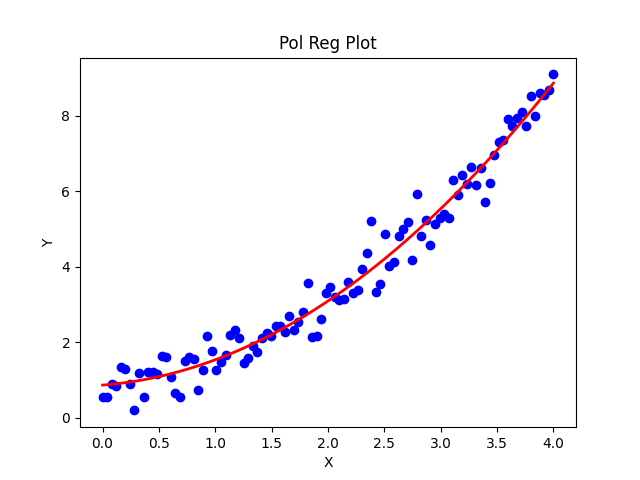
\includegraphics[scale=0.55]{poly_reg.png}\\
      \textbf{figure 1:} image of polynomial regression\\  
    \end{center}
    \item[(e)]
  \end{enumerate}

\end{enumerate}
\end{document}
